\chapter{Evaluation}

In this chapter, we evaluate our version of incremental induced subgraph isomorphism algorithms.

\subsection{Implementation details}

All algorithms were written in Python. Although Python is not necessarily the right tool 
for implementing high performance algorithms, the main goal of this work was to verify if
we can make significant improvements compared to running VF2++/DAF from scratch by computing
mappings incrementally. To evaluate the correctness of our work, two already existing induced 
subgraph isomorphism implementations were used: networkx's (Python graph library) isomorphism 
module and boost c++ library's vf2\_subgraph\_iso module\cite{boostvf2}. Both modules implement VF2. We 
tried to compare the performance against the original VF2++ implementation \cite{lemonvf2pp}
however it did not produce the same results as the selected baseline implementations. We also
wanted to compare our results to the original DAF implementation, however no sources for the
project were available at time of writing, only a set of pre-compiled binaries \cite{dafbin}
which we did not run in the end.

\subsection{Datasets}

We used multiple datasets in our experiments. The first dataset was the Graph Challange\cite{graphchallenge} dataset
which was published by Massachusetts Institute of Technology (MIT) and Amazon Web Services for
the challange. The dataset consists of several large graphs. 

\begin{itemize}
    \item as: network of autonomous systems.
    \item ca-GrQc: collaboration network of general relativity researchers on arxiv.org.
    \item ca-HepTh: collaboration network of high energz physics researchers on arxiv.org.
    \item oregon1: peering infromation of autonomous systems in project Route Views of University of Oregon.
\end{itemize}

The other dataset contains multiple generated graphs, namely scale-free networks generated by the Barabasi-Albert model\cite{barabasimodel}.

\subsection{Measurements}

For each of the graphs, the following operations were made. We ran an initial VF2++ and DAF on the given graph $G$
with query graph defined in figure \ref{fig:expq}. Then we randomly deleted and inserted nodes and edges into $G$,
and we measured how much time does it take to incrementally compute the new mapping set. After the graph modifications
we ran our baseline measurement on the resulting graph $G'$, which was networkx's VF2 implementation and we measured
the time it took for the algorithm to finish. We also verified that the number of ismorphisms found by all algorithms
were the same.

\begin{figure}[h!]
	\centering
	\begin {tikzpicture}[auto, node distance=1cm,thick,main node/.style={circle,draw}]
		\node[main node] (0) {\scriptsize$0$};
		\node[main node] (1) [below left=of 0] {\scriptsize$1$};
		\node[main node] (2) [below right=of 0] {\scriptsize$2$};
		\node[main node] (3) [below=of 1] {\scriptsize$3$};
		\node[main node] (4) [below=of 2] {\scriptsize$4$};
		\draw (0) -- (1);
		\draw (0) -- (2);
		\draw (1) -- (2);
		\draw (2) -- (4);
		\draw (3) -- (4);
		\draw (1) -- (3);
	  \end{tikzpicture}
	\caption{Query graph for our experiments}
	\label{fig:expq}
\end{figure}

The first step of our incremental algorithm is to run VF2++ and DAF from scratch. DAF seems to struggle with more complex queries.
Note that this might be caused by our inefficient implementation. We tried to reach out for the authors of DAF to discuss this issue,
however we did not get any answers. As expected, VF2++ is generally faster than VF2. More importantly, the results verify our proposed 
algorithm in case of VF2++. It is significantly faster to update a graph and incrementally search changes in the mappings than running 
a subgraph ismorphism algorithm from scratch. This applies to all kinds of graphs, even where it takes all three variants a significant
amount of time to find mappings, the incremental version still finishes at least one order of magnitudes earlier.

Figure \ref{fig:evalca} shows the results of our measurements on the ca graphs from Graph Challange. ca-GrQc is special, this was
the only graph where VF2 could beat both initial runs of VF2++ and DAF. It took 20s for VF2 to find all initial 868012 mappings, while
it took 36s and 232s for VF2++ and DAF respectively. However even in this case, the incremental version will outperform the original
in the long run, because adding/removing nodes and edges is so much faster. In this case, incremental VF2++ removed nodes in 0.62s and 
it removed/inserted edges in 7.48s on average. These values were 0.166s and 178s for DAF. The edges to be deleted/inserted were selected 
randomly.

\begin{figure}[h!]
	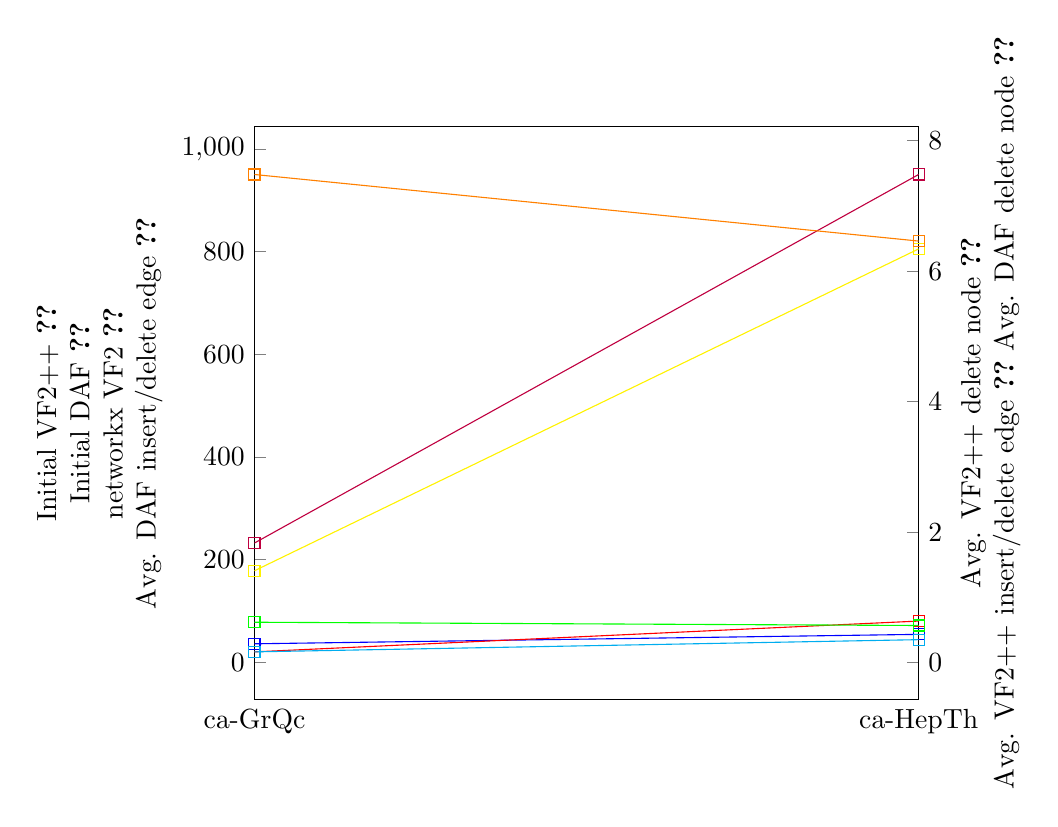
\begin{tikzpicture}
		% let both axes use the same layers
		\pgfplotsset{set layers}
		%
		\begin{axis}[
		scale only axis,
		xmin=0,xmax=1,
		xtick={0,1},
        xticklabels={ca-GrQc,ca-HepTh},
		axis y line*=left,
		ylabel style = {align=center},
		ylabel={Initial VF2++ \ref{plot:vf2ppinitca} \\ Initial DAF \ref{plot:dafinit} \\ networkx VF2 \ref{plot:nxca} \\ Avg. DAF insert/delete edge \ref{plot:dafavginsca}},
		]
		\addplot[
            color=blue,
            mark=square,
            ]
            coordinates {
            (0,35.7)(1,54.1)
            };
			\label{plot:vf2ppinitca}
		\addplot[
			color=purple,
			mark=square,
			]
			coordinates {
			(0,232)(1,950)
			};
			\label{plot:dafinit}
		\addplot[
			color=red,
			mark=square,
			]
			coordinates {
			(0,20)(1,80)
			};
			\label{plot:nxca}
		\addplot[
			color=yellow,
			mark=square,
			]
			coordinates {
			(0,178)(1,805)
			};
			\label{plot:dafavginsca}

		\end{axis}
		%
		\begin{axis}[
		scale only axis,
		xmin=0,xmax=1,
		axis y line*=right,
		axis x line=none,
		ylabel style = {align=center},
		ylabel={Avg. VF2++ delete node \ref{plot:avgnodeca} \\ Avg. VF2++ insert/delete edge \ref{plot:avginsca} Avg. DAF delete node \ref{plot:dafavgnodeca}},
		]
		\addplot[
			color=green,
            mark=square,
            ]
            coordinates {
            (0,0.62)(1,0.57)
            };
            \label{plot:avgnodeca}
        \addplot[
			color=orange,
            mark=square,
            ]
            coordinates {
            (0,7.48)(1,6.46)
            };
            \label{plot:avginsca}

		\addplot[
			color=cyan,
			mark=square,
			]
			coordinates {
			(0,0.166)(1,0.353)
			};
			\label{plot:dafavgnodeca}		
		\end{axis}
		%
		\end{tikzpicture}
		\caption{Results of ca graphs from Graph Challange}
		\label{fig:evalca}
\end{figure}

\begin{table}[h!]
	\centering
	\def\arraystretch{1.2}
	\begin{tabular}{c|c|c|c}
	\hline
	Algorithm     & Initial  & Node deletion & Edge deletion    \\ \hline \hline
	VF2++         & 35.7s  & 0.62s     & 7.48s \\ \hline
	DAF           & 232s  & 0.166s   & 178s \\ \hline
	networkx.VF2  & 20s  & N/A     & N/A \\ \hline
	\end{tabular}

	\caption{Table showing results of ca-GrQc}
\end{table}

The oregon graphs from Graph Challange were the largest and this were the graphs where the incremental version really shined.
To find the initial 3,568,766 mappings in oregon\_010331, it took 1595s, 7106s, and 4896s for VF2++, DAF and VF2 respectively. 
In case of node deletion and edge insertion/deletion, incremental VF2++ was able to update the set of mappings in 37.6s and 179.5s.
Incremental DAF was able to delete nodes in 2.51s but it took almost as much time (4133s) to update the mappings in case of edge
insertions as its initial run. There are missing DAF results for the other two oregon graphs. This is because it did not finish in 10,000s.

\begin{figure}[h!]
	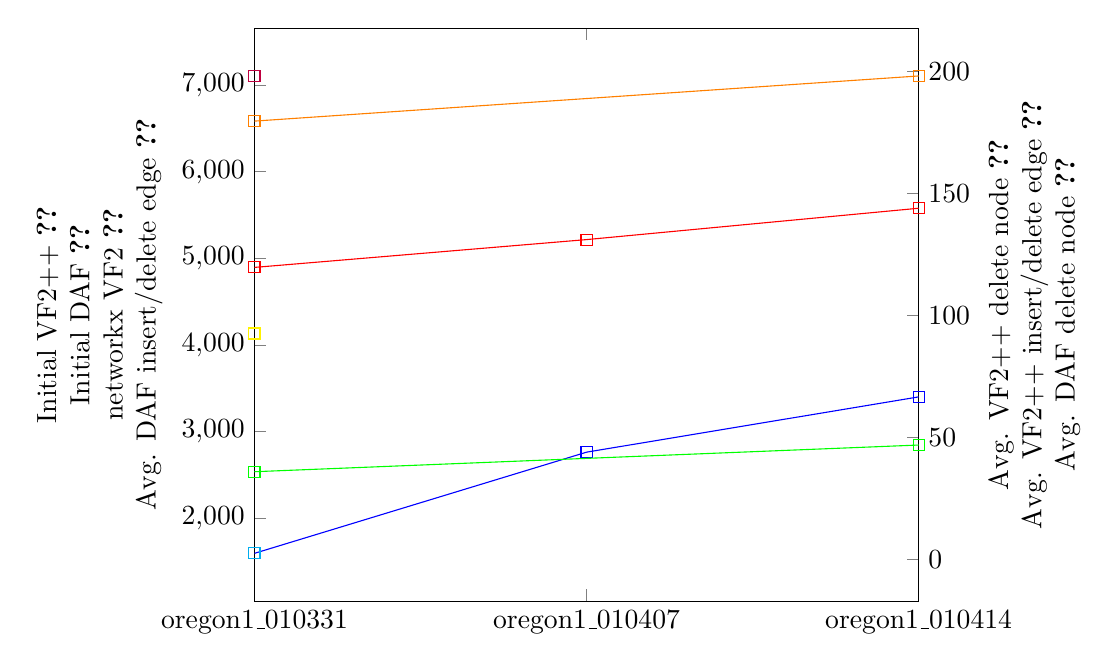
\begin{tikzpicture}
		% let both axes use the same layers
		\pgfplotsset{set layers}
		%
		\begin{axis}[
		scale only axis,
		xmin=0,xmax=2,
		xtick={0,1,2},
        xticklabels={oregon1\_010331,oregon1\_010407, oregon1\_010414},
		axis y line*=left,
		ylabel style = {align=center},
		ylabel={Initial VF2++ \ref{plot:vf2ppinitoregon} \\ Initial DAF \ref{plot:dafinitoregon} \\ networkx VF2 \ref{plot:nxoregon} \\ Avg. DAF insert/delete edge \ref{plot:dafavginsoregon}},
		]
		\addplot[
            color=blue,
            mark=square,
            ]
            coordinates {
            (0,1595)(1,2763)(2,3401)
            };
			\label{plot:vf2ppinitoregon}
		\addplot[
			color=purple,
			mark=square,
			]
			coordinates {
			(0,7106)
			};
			\label{plot:dafinitoregon}
		\addplot[
			color=red,
			mark=square,
			]
			coordinates {
			(0,4896)(1,5217)(2,5579)
			};
			\label{plot:nxoregon}		
		\addplot[
			color=yellow,
			mark=square,
			]
			coordinates {
			(0,4133)
			};
			\label{plot:dafavginsoregon}
		\end{axis}
		%
		\begin{axis}[
		scale only axis,
		xmin=0,xmax=1,
		axis y line*=right,
		axis x line=none,
		ylabel style = {align=center},
		ylabel={Avg. VF2++ delete node \ref{plot:avgnodeoregon} \\ Avg. VF2++ insert/delete edge \ref{plot:avginsoregon} \\ Avg. DAF delete node \ref{plot:dafavgnodeoregon}},
		]
		\addplot[
			color=green,
            mark=square,
            ]
            coordinates {
            (0,35.94)(1,46.87)(2,58.77)
            };
            \label{plot:avgnodeoregon}
        \addplot[
			color=orange,
            mark=square,
            ]
            coordinates {
            (0,179.54)(1,198.03)(2,236.77)
            };
            \label{plot:avginsoregon}
		\addplot[
			color=cyan,
			mark=square,
			]
			coordinates {
			(0,2.511)
			};
			\label{plot:dafavgnodeoregon}		
		\end{axis}
		%
		\end{tikzpicture}
		\caption{Results of oregon graphs from Graph Challange}
\end{figure}

\begin{table}[h!]
	\centering
	\def\arraystretch{1.2}
	\begin{tabular}{c|c|c|c}
	\hline
	Algorithm     & Initial  & Node deletion & Edge deletion    \\ \hline \hline
	VF2++         & 1595s  & 35.94s  & 179.54s \\ \hline
	DAF           & 7106s  & 2.51s   & 4133s \\ \hline
	networkx.VF2  & 4896s  & N/A     & N/A \\ \hline
	\end{tabular}

	\caption{Table showing results of oregon-010331}
\end{table}

Incremental VF2++ was also the fastest in case of scale-free graphs. We can see that it took roughly $1/10$-th of VF2's time for VF2++ to finish
its initial run, and it took roughly $1/10$-th of the time of VF2++'s initial run for the incremental algorithm to find the new set of mappings
in a modified graph. DAF performed similarly poorly as in previous cases.

\begin{figure}
	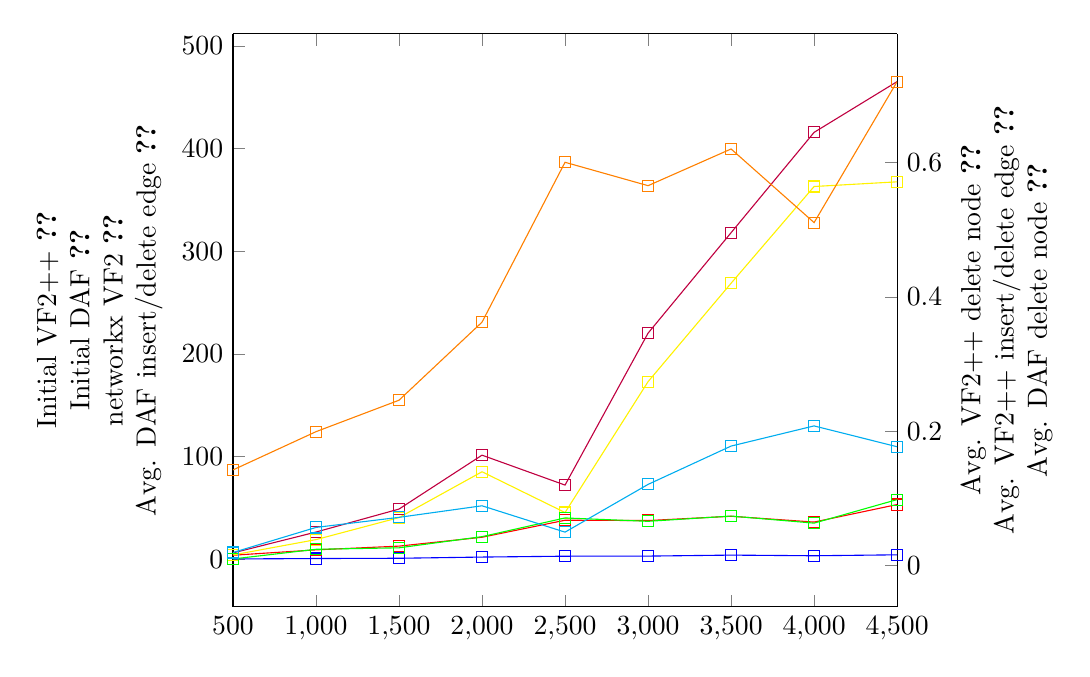
\begin{tikzpicture}
		% let both axes use the same layers
		\pgfplotsset{set layers}
		%
		\begin{axis}[
		scale only axis,
		xmin=500,xmax=4500,
		xtick={500,1000,...,4500},
		axis y line*=left,
		ylabel style = {align=center},
		ylabel={Initial VF2++ \ref{plot:vf2ppinitbar} \\ Initial DAF \ref{plot:dafbar} \\ networkx VF2 \ref{plot:nxbar} \\ Avg. DAF insert/delete edge \ref{plot:dafavginsbar}},
		]
		\addplot[
            color=blue,
            mark=square,
            ]
            coordinates {
            (500,0.34)(1000,0.77)(1500,1.02)(2000,2.19)(2500,3.03)(3000,3.13)(3500,4.096)(4000,3.46)(4500,4.38)
            };
			\label{plot:vf2ppinitbar}
		\addplot[
			color=purple,
			mark=square,
			]
			coordinates {
			(500,6.22)(1000,26.54)(1500,48.92)(2000,101.41)(2500,72.28)(3000,220.2)(3500,318.04)(4000,415.72)(4500,465.15)
			};
			\label{plot:dafbar}		
		\addplot[
			color=red,
			mark=square,
			]
			coordinates {
			(500,3.97)(1000,9.2)(1500,12.85)(2000,21.48)(2500,38.05)(3000,37.74)(3500,41.91)(4000,36.26)(4500,53.33)
			};
			\label{plot:nxbar}		
		\addplot[
			color=yellow,
			mark=square,
			]
			coordinates {
			(500,4.25)(1000,19.18)(1500,40.62)(2000,85.25)(2500,45.55)(3000,172.98)(3500,268.81)(4000,363)(4500,367.56)
			};
			\label{plot:dafavginsbar}  
		\end{axis}
		%
		\begin{axis}[
		scale only axis,
		xmin=500,xmax=4500,
		axis y line*=right,
		axis x line=none,
		ylabel style = {align=center},
		ylabel={Avg. VF2++ delete node \ref{plot:avgnodebar} \\ Avg. VF2++ insert/delete edge \ref{plot:avginsbar} \\ Avg. DAF delete node \ref{plot:dafavgnodebar}},
		]
		\addplot[
			color=green,
            mark=square,
            ]
            coordinates {
            (500,0.0101)(1000,0.0245)(1500,0.02669)(2000,0.0433)(2500,0.0711)(3000,0.0661)(3500,0.0739)(4000,0.0634)(4500,0.0984)
            };
            \label{plot:avgnodebar}
		\addplot[
			color=orange,
			mark=square,
			]
			coordinates {
			(500,0.1425)(1000,0.1994)(1500,0.2462)(2000,0.3623)(2500,0.6001)(3000,0.5653)(3500,0.6199)(4000,0.5104)(4500,0.7201)
			};
			\label{plot:avginsbar}    
		\addplot[
			color=cyan,
            mark=square,
            ]
            coordinates {
            (500,0.0197)(1000,0.057)(1500,0.072)(2000,0.0892)(2500,0.05)(3000,0.121)(3500,0.178)(4000,0.208)(4500,0.177)
            };
            \label{plot:dafavgnodebar}		
		\end{axis}
		%
		\end{tikzpicture}
		\caption{Results of scale-free graphs generated by Barabasi-model}
\end{figure}

\begin{table}[h!]
	\centering
	\def\arraystretch{1.2}
	\begin{tabular}{c|c|c|c}
	\hline
	Algorithm     & Initial  & Node deletion & Edge deletion    \\ \hline \hline
	VF2++         & 4.38s  & 0.0984s     & 0.7201s \\ \hline
	DAF           & 465.15s  & 0.177s   & 367.56s \\ \hline
	networkx.VF2  & 53.33s  & N/A     & N/A \\ \hline
	\end{tabular}

	\caption{Table showing results of a scale-free graph with 4500 nodes and 13500 edges}
\end{table}